\appendix
\pagenumbering{Roman}
\chapter*{Přílohy}

\section*{A. Zdrojový kód aplikace zobrazující hostname\label{app:hostname}}
\begin{verbatim}
package main

import (
        "fmt"
        "log"
        "net/http"
        "os"
       )

func handler(w http.ResponseWriter, r *http.Request) {
        name, err := os.Hostname()
        if err != nil{
                log.Println("Unable to retrieve hostname")
        }
        fmt.Fprintf(w, "HOSTNAME: %s",name)
}

func main() {
        http.HandleFunc("/",handler)
        log.Fatal(http.ListenAndServe(":80",nil))
}
\end{verbatim}


\clearpage
\section*{B. Zdrojový kód aplikace zobrazující soubory v definovaném adresáři\label{app:servefiles}}
\begin{verbatim}
package main

import (
	"log"
	"net/http"
	"os"
	"time"
)

const directoryToServe = "/tmp"

func main() {
	path := os.Getenv("DIRECTORY_PATH")
	if path == ""{
		path = directoryToServe
	}
	log.Printf("Serving directory %s",path)
	hostname, err := os.Hostname()
	if err != nil{
		log.Printf("Cannot get hostname")
	}
	time := time.Now().Format(time.RFC3339)
	fileName := path+"/"+hostname+"-"+time
	newFile,err := os.Create(fileName)
	if err != nil {
		log.Printf("unable to create a file, %s",err)
	}
	log.Printf("New file created: %s", newFile.Name())

	fs := http.FileServer(http.Dir(path))
	http.Handle("/", fs)
	log.Println("Serving files on port 3000")
	http.ListenAndServe(":3000", nil)
}
\end{verbatim}


\clearpage
\section*{C. Manifest pro vytvoření statefulsetu\label{app:statefulset}}
\begin{verbatim}
apiVersion: v1
kind: Secret
metadata:
 name: secretenv
type: Opaque
data:
  dirpath: L2RpcGxvbWthLXNlcnZlLWZpbGVz
---
apiVersion: apps/v1
kind: StatefulSet
metadata:
  name: fileserver
spec:
  serviceName: "fileserver-service"
  replicas: 2
  selector:
    matchLabels:
      app: fileserver
  template:
    metadata:
      labels:
        app: fileserver
    spec:
      containers:
      - name: fileserver
        image: casek14/diplomka-servefiles
        ports:
        - containerPort: 3000
          name: servefiles
        volumeMounts:
        - name: serverdir
          mountPath: /diplomka-serve-files
        env:
        - name: DIRECTORY_PATH
          valueFrom:
            secretKeyRef:
              name: secretenv
              key: dirpath
  volumeClaimTemplates:
  - metadata:
      name: serverdir
    spec:
      accessModes: [ "ReadWriteOnce" ]
      storageClassName: "minikube-class"
      resources:
        requests:
          storage: 1Gi
---
apiVersion: v1
kind: Service
metadata:
  name: serve-file-service
spec:
  selector:
    app: fileserver
  type: NodePort
  ports:        
  - protocol: TCP
    port: 8080
    targetPort: 3000
\end{verbatim}

\clearpage
\section*{D. Struktura aplikace\label{app:struktura}}
\begin{figure}[H]
  %\begin{centering}
    
	  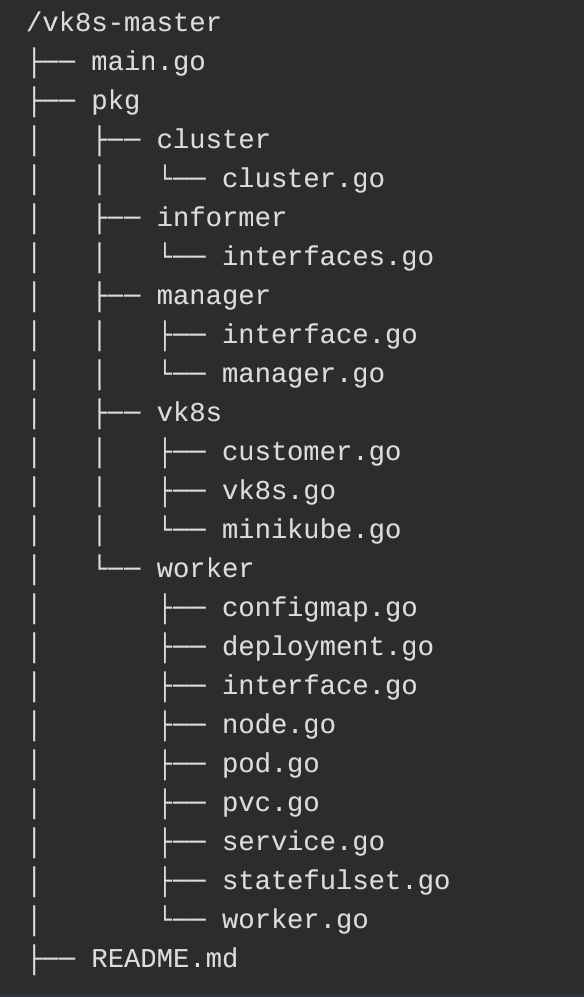
\includegraphics[width=0.5\textwidth]{images/vk8s-master.png}
   %\end{centering}
\end{figure}
%\begin{lstlistin}
%/vk8s-master\newline
%|---main.go\newline
%|---pkg\newline
%|   |---cluster\newline
%|   |   '---cluster.go\newline
%|   |---informer\newline
%|   |   '---interfaces.go\newline
%|   |---manager\newline
%|   |   |---interface.go\newline
%|   |   '---manager.go\newline
%|   |---vk8s\newline
%|   |   |---customer.go\newline
%|   |   |---vk8s.go\newline
%|   |   '---minikube.go\newline
%|   '---worker\newline
%|       |---configmap.go\newline
%|       |---deployment.go\newline
%|       |---interface.go\newline
%|       |---node.go\newline
%|       |---pod.go\newline
%|       |---pvc.go\newline
%|       |---service.go\newline
%|       |---statefulset.go\newline
%|       '---worker.go\newline
%|---README.md
%
%\end{lstlisting}
